\documentclass[dvipsnames]{beamer}
\usetheme{CambridgeUS}

\usepackage{minted}
\usepackage{mathspec}
\usepackage{xcolor}

\usepackage{tikz}
\usetikzlibrary{calc,shapes.multipart,chains,arrows}

\setmainfont[Ligatures=TeX]{XITS}
\setmathfont{XITS Math}

\title{agdARGS}
\subtitle{Command Line Arguments, Options and Flags}
\author[G. Allais]{Guillaume Allais}
\institute[Strathclyde]{University of Strathclyde}
\date[IDM, March 2015]{Idris Developers Meeting, March 2015}

\begin{document}

\begin{frame}
 \maketitle
\end{frame}

\section{Motivation}
\subsection{Let's compile!}

\begin{frame}
 \frametitle{Crazy thought: let's compile some programs!}

  Bored of the stereotype that in Type Theory we never go anywhere
  past typechecking or producing \texttt{.tex} documents (which,
  by the way, Travis can help with! \url{http://blog.gallais.org/travis-builds}).

  \vspace{0.7cm}

  Decided to build a simple executable because I can.
\end{frame}

\subsection{aGdaREP}

\begin{frame}{\url{https://github.com/gallais/aGdaREP}}

  My simple pick: a certified regexp matcher leading to an
  implementation of \texttt{grep}.

 \begin{center}
   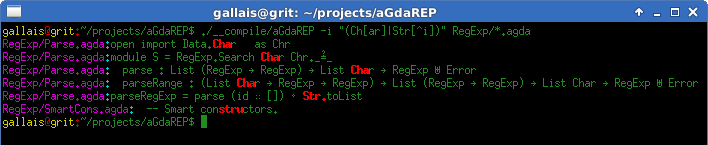
\includegraphics[width=0.9\textwidth]{screenshot.png}
 \end{center}

  Lots of fun implementing, optimizing and extending the correct by
  construction matcher (see Alexandre Agular and Bassel Mannaa's 2009
  "Regular Expressions in Agda" ),

  But... then we need a user-facing interface!
\end{frame}

\begin{frame}[fragile]{A cheeky account of my journey}

  First step: add a binding to the important \texttt{Haskell}
  function...

\begin{minted}{haskell}
module Bindings.Arguments.Primitive where

open import IO.Primitive
open import Data.List
open import Data.String

{-# IMPORT System.Environment #-}

postulate
  getArgs : IO (List String)

{-# COMPILED getArgs System.Environment.getArgs #-}

\end{minted}
\end{frame}

\begin{frame}[fragile]{But wait! There's more!}

  Then lift the bound primitive to the \texttt{IO} type actually used
  at a high level of abstraction:

\begin{minted}{haskell}
module Bindings.Arguments where

open import Data.List
open import Data.String
open import IO
import Bindings.Arguments.Primitive as Prim

getArgs : IO (List String)
getArgs = lift Prim.getArgs
\end{minted}

  I guess it's a good way to learn about the language's and the
  standard library's internals? Which, maybe, I did not want to.
  Anyway.
\end{frame}

\begin{frame}[fragile]{"Hand-crafted" solution}

Now that we have access to the arguments, we just have to make sense
of them. We use a type of options:

\begin{minted}{haskell}
record grepOptions : Set where
  field
    -V     : Bool            -- version
    -v     : Bool            -- invert match
    -i     : Bool            -- ignore case
    regexp : Maybe String    -- regular expression
    files  : List FilePath   -- list of files to mine
open grepOptions public
\end{minted}

And "hand-craft" a function populating it:
\end{frame}

\begin{frame}[fragile]
\begin{minted}{haskell}
parseOptions : List String -> grepOptions
parseOptions args =
  record result { files = reverse (files result) }
  where
    cons : grepOptions -> String -> grepOptions
    cons opt "-v" = record opt { -v = true }
    cons opt "-V" = record opt { -V = true }
    cons opt "-i" = record opt { -i = true }
    cons opt str  =
      if is-nothing (regexp opt)
      then record opt { regexp = just str }
      else record opt { files  = str :: files opt }

    result : grepOptions
    result = foldl cons defaultGrepOptions args
\end{minted}
\end{frame}

\begin{frame}[fragile]{A few issues}
  \begin{itemize}
    \item I don't want to have to write this for every app
    \item This is not even ready for consumption yet!
      \begin{minted}{haskell}
       regexp : Maybe String
      \end{minted}
  \end{itemize}
\end{frame}

\section{Design the internals}
\subsection{Types}

\begin{frame}{What is a command-line interface?}

  \begin{itemize}
    \item A set of \emph{distinct} flag or options
    \item Each potentially coming with an \emph{argument}
    \item Living in a \emph{domain} of values
    \item We know how to \emph{parse}
  \end{itemize}
\end{frame}

\begin{frame}[fragile]{The (minimal) type of an \texttt{Argument}}
\begin{minted}{haskell}
record Argument (l : Level) : Set (suc l) where
  field
    flag        : String
    domain      : Domain l
    parser      : parserType domain

data Domain (l : Level) : Set (suc l) where
  None :                     Domain l
  Some : (S : Set l)      -> Domain l
  ALot : (M : RawMagma l) -> Domain l

parserType : {l : Level} -> Domain l -> Set l
parserType None     = Lift Unit
parserType (Some S) = String -> String || S
parserType (ALot M) = String -> String || carrier M
\end{minted}
\end{frame}

\begin{frame}[fragile]
  A CLI is defined by an \textbf{extensible record} of arguments.

  \begin{itemize}
    \item guaranteed uniqueness of flags
    \item easy to lookup values
    \item easy to extend
    \item first class citizens (generic programming possible!)
  \end{itemize}
\end{frame}

\subsection{Types - Keep your neighbours in order}

\begin{frame}{The type of extensible records}
  McBride to the rescue: How to keep your neighbours in order

  The special case of lists, using a \emph{strict} total order:
%%%%%%%%%%%%%%%%%%%%%%%%%%%%%%%%%%%%%%%%%%%%%%%%%%%%%%%%%%%%
%%%%%%%%%%%%%%%%%%%%%%%%%%%%%%%%%%%%%%%%%%%%%%%%%%%%%%%%%%%%
\begin{figure}[t]
\centering
\begin{tikzpicture}[list/.style={rectangle split, rectangle split parts=2,
    draw, rectangle split horizontal}, >=stealth, start chain]

  \node[list,on chain] (A) {{\color{red}-$\infty$} < {\color{ForestGreen}12}};
  \node[list,on chain] (B) {{\color{gray}12} < {\color{ForestGreen}99}};
  \node[list,on chain] (C) {{\color{gray}99} < {\color{ForestGreen}128}};
  \node[on chain,draw] (D) {{\color{gray}128} < {\color{red}+$\infty$}};
  \draw[*->] let \p1 = (A.two), \p2 = (A.center) in (\x1,\y2) -- (B);
  \draw[*->] let \p1 = (B.two), \p2 = (B.center) in (\x1,\y2) -- (C);
  \draw[*->] let \p1 = (C.two), \p2 = (C.center) in (\x1,\y2) -- (D);
\end{tikzpicture}
\end{figure}

%%%%%%%%%%%%%%%%%%%%%%%%%%%%%%%%%%%%%%%%%%%%%%%%%%%%%%%%%%%%%%%%%%%%
%%%%%%%%%%%%%%%%%%%%%%%%%%%%%%%%%%%%%%%%%%%%%%%%%%%%%%%%%%%%%%%%%%%%
\end{frame}

\begin{frame}[fragile]
  \begin{minted}{haskell}
  data USL (lb ub : Carrier) : Set _ where
    []     : lb < ub -> USL lb ub
    _,_::_ : hd (lt : lb < emb hd) (tl : USL (emb hd) ub) ->
             USL lb ub
  \end{minted}
\end{frame}

\begin{frame}
\end{frame}

\subsection{Terms}

\begin{frame}[fragile]
Jon Sterling to the rescue: "Vinyl: Modern Records for Haskell."

\begin{minted}{haskell}
  Mode : (args : USL lb ub) -> Set (suc l)
  Mode args = arg (pr : arg inUSL args) -> Set l

  options : (args : USL lb ub) (m : Mode args) -> Set l
  options []                m = Lift 1
  options (hd , lt :: args) m = m hd z * options args _

\end{minted}

\end{frame}

\begin{frame}
\end{frame}

\section{Design a nice interface}
\begin{frame}[fragile]{We can \textbf{run} an awful lot at \textbf{compile time}}
Our users will only ever use concrete CLI descriptions. As such, a
lot of the decision procedure can be run at compile time thus offering
a nicer interface.

\end{frame}


\end{document}
